\documentclass[12pt,a4paper]{report}
\usepackage[utf8]{inputenc}
\usepackage{amsmath}
\usepackage{amsfonts}
\usepackage{amssymb}
\usepackage{amsthm}
\usepackage{hyperref}

\usepackage{multicol}
\usepackage{fancyhdr}
\usepackage[inline]{enumitem}
\usepackage{tikz}
\usepackage{tikz-cd}
\usetikzlibrary{calc}
\usetikzlibrary{shapes.geometric}
\usepackage[margin=0.5in]{geometry}
\usepackage{xcolor}
\usepackage{listings} 

\hypersetup{
    colorlinks=true,
    linkcolor=blue,
    filecolor=magenta,      
    urlcolor=cyan,
    pdftitle={Tensors},
    pdfpagemode=FullScreen,
    }

%\urlstyle{same}

\newcommand{\CLASSNAME}{Math 5315 -- Numerical Methods for PDE}
\newcommand{\STUDENTNAME}{Paul Carmody}
\newcommand{\ASSIGNMENT}{Midterm Project }
\newcommand{\DUEDATE}{November 12, 2025}
\newcommand{\SEMESTER}{Fall 2025}
\newcommand{\SCHEDULE}{TTh 2:00 to 3:15}
\newcommand{\ROOM}{Crawford 111}

\newcommand{\MMN}{M_{m\times n}}
\newcommand{\FF}{\mathcal{F}}

\pagestyle{fancy}
 	\fancyhf{}
\chead{ \fancyplain{}{\CLASSNAME} }
%\chead{ \fancyplain{}{\STUDENTNAME} }
\rhead{\thepage}
\input{../MyMacros}

\newcommand{\RED}[1]{\textcolor{red}{\#1}}
\newcommand{\BLUE}[1]{\textcolor{blue}{\#1}}
\definecolor{mygreen}{RGB}{28,172,0} % color values Red, Green, Blue
\definecolor{mylilas}{RGB}{170,55,241}

\begin{document}
\lstset{language=Matlab,%
    %basicstyle=\color{red},
    breaklines=true,%
    morekeywords={matlab2tikz},
    keywordstyle=\color{blue},%
    morekeywords=[2]{1}, keywordstyle=[2]{\color{black}},
    identifierstyle=\color{black},%
    stringstyle=\color{mylilas},
    commentstyle=\color{mygreen},%
    showstringspaces=false,%without this there will be a symbol in the places where there is a space
    numbers=left,%
    numberstyle={\tiny \color{black}},% size of the numbers
    numbersep=9pt, % this defines how far the numbers are from the text
    emph=[1]{for,end,break},emphstyle=[1]\color{red}, %some words to emphasise
    %emph=[2]{word1,word2}, emphstyle=[2]{style},    
}

\begin{center}
	\Large{\CLASSNAME -- \SEMESTER} \\
	\large{ w/Professor Du}
\end{center}
\begin{center}
	\STUDENTNAME \\
	\ASSIGNMENT -- \DUEDATE\\
\end{center} 
\HLINE

\begin{center}
	\textbf{\Large{Apply the FTFS scheme to the\\ Wave Equation with Periodic Boundary Conditions}}
\end{center}

\begin{description}
	\item \textbf{FTFS over the Wave Function:}
	
	Given the Wave Equation with periodic boundary conditions over $[0,1]$, that is
	\begin{align*}
		\BINDEF{u_{t}-u_{x} = 0 & x \in [0,1], \, t > 0}{u(x,0) = u(x,1) = 1.} & (1)
	\end{align*}The FTFS scheme works by evenly dividing the time and spatial dimensions separating points by $\Delta t$ and $\Delta x$, not necessarily equal. Thus, each point over the domain can be calculated at $u_j^{k+1} = u_j^k + \Delta t$ and $u_{j+1}^{k} = u_j^k + \Delta x$.  Then, by applying the forward time difference we approximate the derivative at each point.
$$\frac{\partial u}{\partial t} \approx \frac{u_j^{n+1} - u_j^n}{\Delta t} + O(\Delta t).$$ Then, applying the forward-space difference, the spatial derivative, 
$$\frac{\partial u}{\partial x} \approx \frac{u_{j+1}^n - u_j^n}{\Delta x} + O(\Delta x)$$.

Substituting these finite difference approximations into the wave equation (1):
$$\frac{u_j^{n+1} - u_j^n}{\Delta t} +  \frac{u_{j+1}^n - u_j^n}{\Delta x} = 0$$
Solving for $u_j^{n+1}$ in order to calculate successive points,
$$u_j^{n+1} = u_j^n - \frac{\Delta t}{\Delta x} (u_{j+1}^n - u_j^n)$$

We can then interate over both the time and spatial dimensions via $\Delta t$ and $\Delta x$ to provide successive data points.  It will be convenient to introduce  the Courant-Fredrichs-Lewey number, $\lambda$ as 
\begin{align*}
	\lambda &= \frac{\Delta t}{\Delta x}
\end{align*}and consequently
\begin{align}
	u_j^{n+1} &= (1+\lambda)u_j^n-\lambda u_{j+1}^n
\end{align}

%%% insert graph of analytic vs numerical solutions here.
\newpage
\textbf{Analytic vs Numerical solutions}

\begin{figure}[h!]
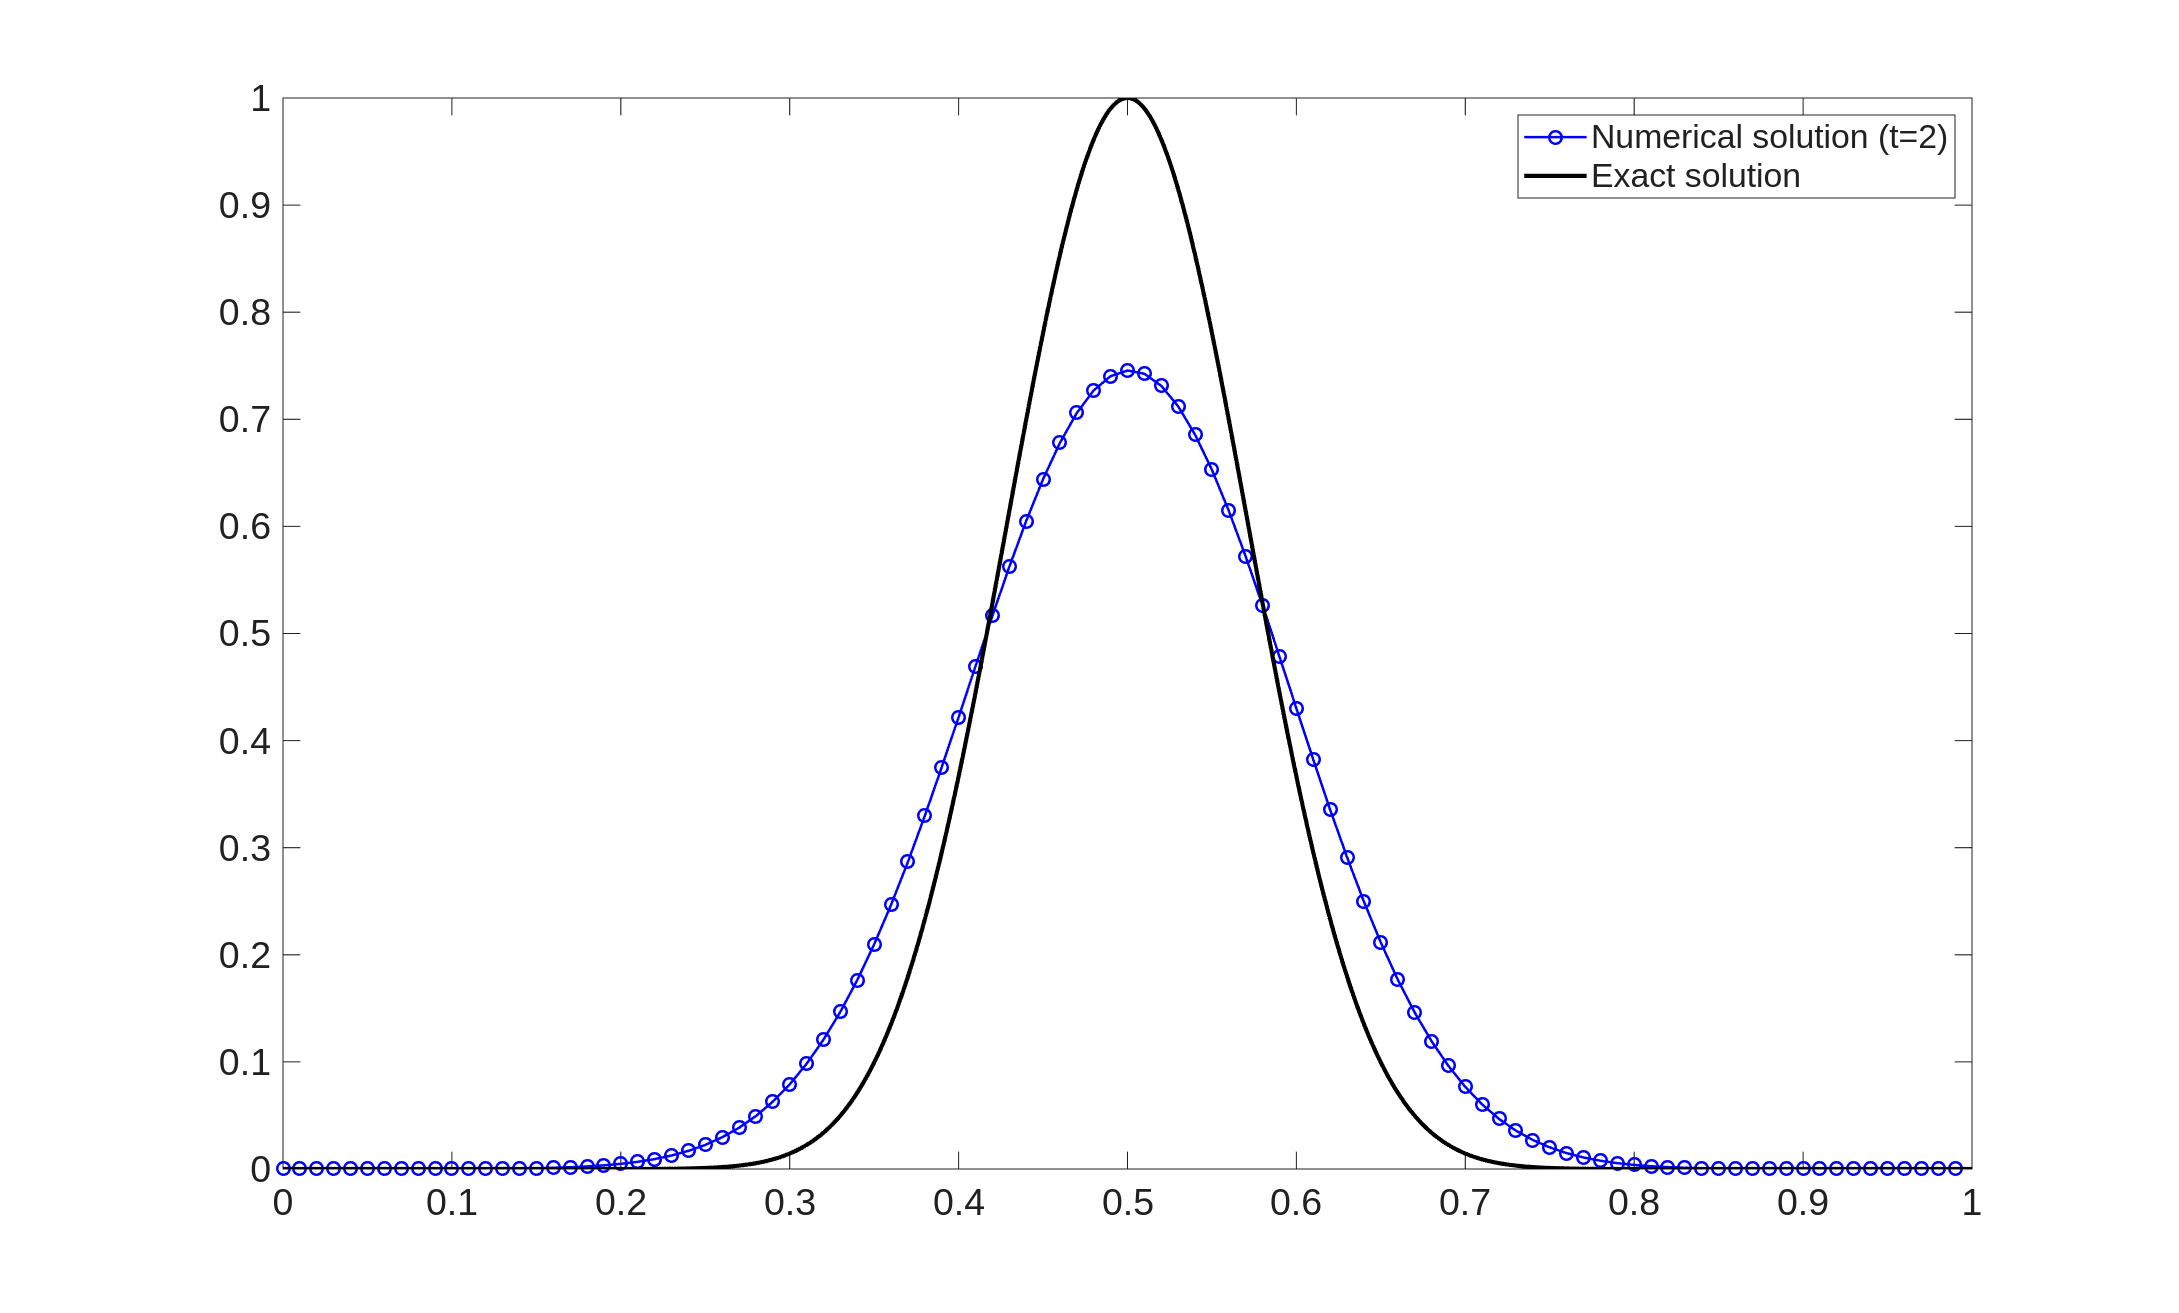
\includegraphics[scale=0.5]{AnaVsNum.png} 
\caption{Analytic vs Numerical Solution}
\label{fig:Graph1}
\end{figure}



%%% inset code for the graph.
Here is the MatLab code that generated the graph.

\label{OriginalCode}
\lstinputlisting{upwind.m}

Now let's draw attention to line 52 which encodes the FTFS expression.  Further, the graph shows a dampened amplitude in the wave along with ``softened" base, i.e., spreadout slightly near the horizontal axis.  One might consider if the areas under each curve are the same.\\

Now see line 66 which calls ``exactsolution" which is the analytic solution.  Its code is here
\lstinputlisting{exactsolution.m}

The commented out portions will be used in part (c) of the assignment.
	
	\item \textbf{Dispersion and Dissipation}
	\begin{description}
		\item \textbf{Dispersion}
		
		We should consider our wave as made up of wave components, i.e., a series of pure wave expressions.  The PDE dictates that all wave components should travel at the same speed.  This, however, is where numerical approximation can deviate from the analytical expression.  This deviation is called \textit{dispersion} and is cumulative over the interval of interest.  The effect is that the shape of the wave spreads out over time as seen in Figure \ref{fig:Graph1}.  \\
		
		The term 'wave components' indicates Fourier Analysis.  In light of equation (1) we look towards a solution of the form
		\begin{align*}
			u_j^n &= \hat{u}^ne^{ij\theta}
		\end{align*}where $j$ is the discrete spatial index with $\Delta x$ giving $j\theta$.  Applying this to (1) we obtain 
		\begin{align*}
			\hat{u}^{n+1}e^{ij\theta} &= (1+\lambda)\hat{u}^ne^{ij\theta}-\lambda \hat{u}^ne^{i(j+1)\theta} \\
			\hat{u}^{n+1} &= (1+\lambda)\hat{u}^n-\lambda \hat{u}^ne^{i\theta} \\
			\frac{\hat{u}^{n+1}}{\hat{u}^n} &= (1+\lambda)-\lambda e^{i\theta}
		\end{align*}With a small $\lambda$ this demonstrates that each iteration has an increasing value over $n$ ($\theta$ depends on $n$) and effected by the wave number.  We'll define $G(\theta)$ as 
		\begin{align*}
			G(\theta) &= (1+\lambda)-\lambda e^{i\theta} = \frac{u^{n+1}}{u^n} 
		\end{align*}
		
		\item \textbf{Dissipation}
		
		In addition to a dispersion of wave speeds over interations in numerical methods is the potential to effect the amplitude of the wave.  We define this effect as \textit{dissipation}.  The ideal case, is that there is no dissipation then, of course, to minimize the effect that iterative solutions can introduce.  Since it is an iterative solution, this, too, can be cumulative.\\
		
		We can see that the ratio between successive iterations, $|G(\theta)|$, effects the progressive amplitude.  That is, $|G(\theta)| = 1$ indicates no dissipation, $|G(\theta)| < 1$ implies a decaying amplitude and $|G(\theta)| > 1$ indicates an unstable scheme.
		
		\item \textbf{Indicators for Dispersion and Dissipation}
		
		Intuitively, the best indicator for dissipation would be to observe the effect of $G(\theta)$ over $\theta$.  This will indicate the effect of wave number on the dissipative effect.  However, for dispersion an appropriate indicator would be to compare the appoximation of the wave component, $\omega(k)$, with the numerical approximation, $\bar{\omega}(k)$ where $k$ is the wave number.
		\begin{align*}
			\omega(k) &= - |G(\theta)|/\Delta t \\
			\bar{\omega}(k) &= -\theta/\Delta t
		\end{align*}
		
		\begin{figure}
			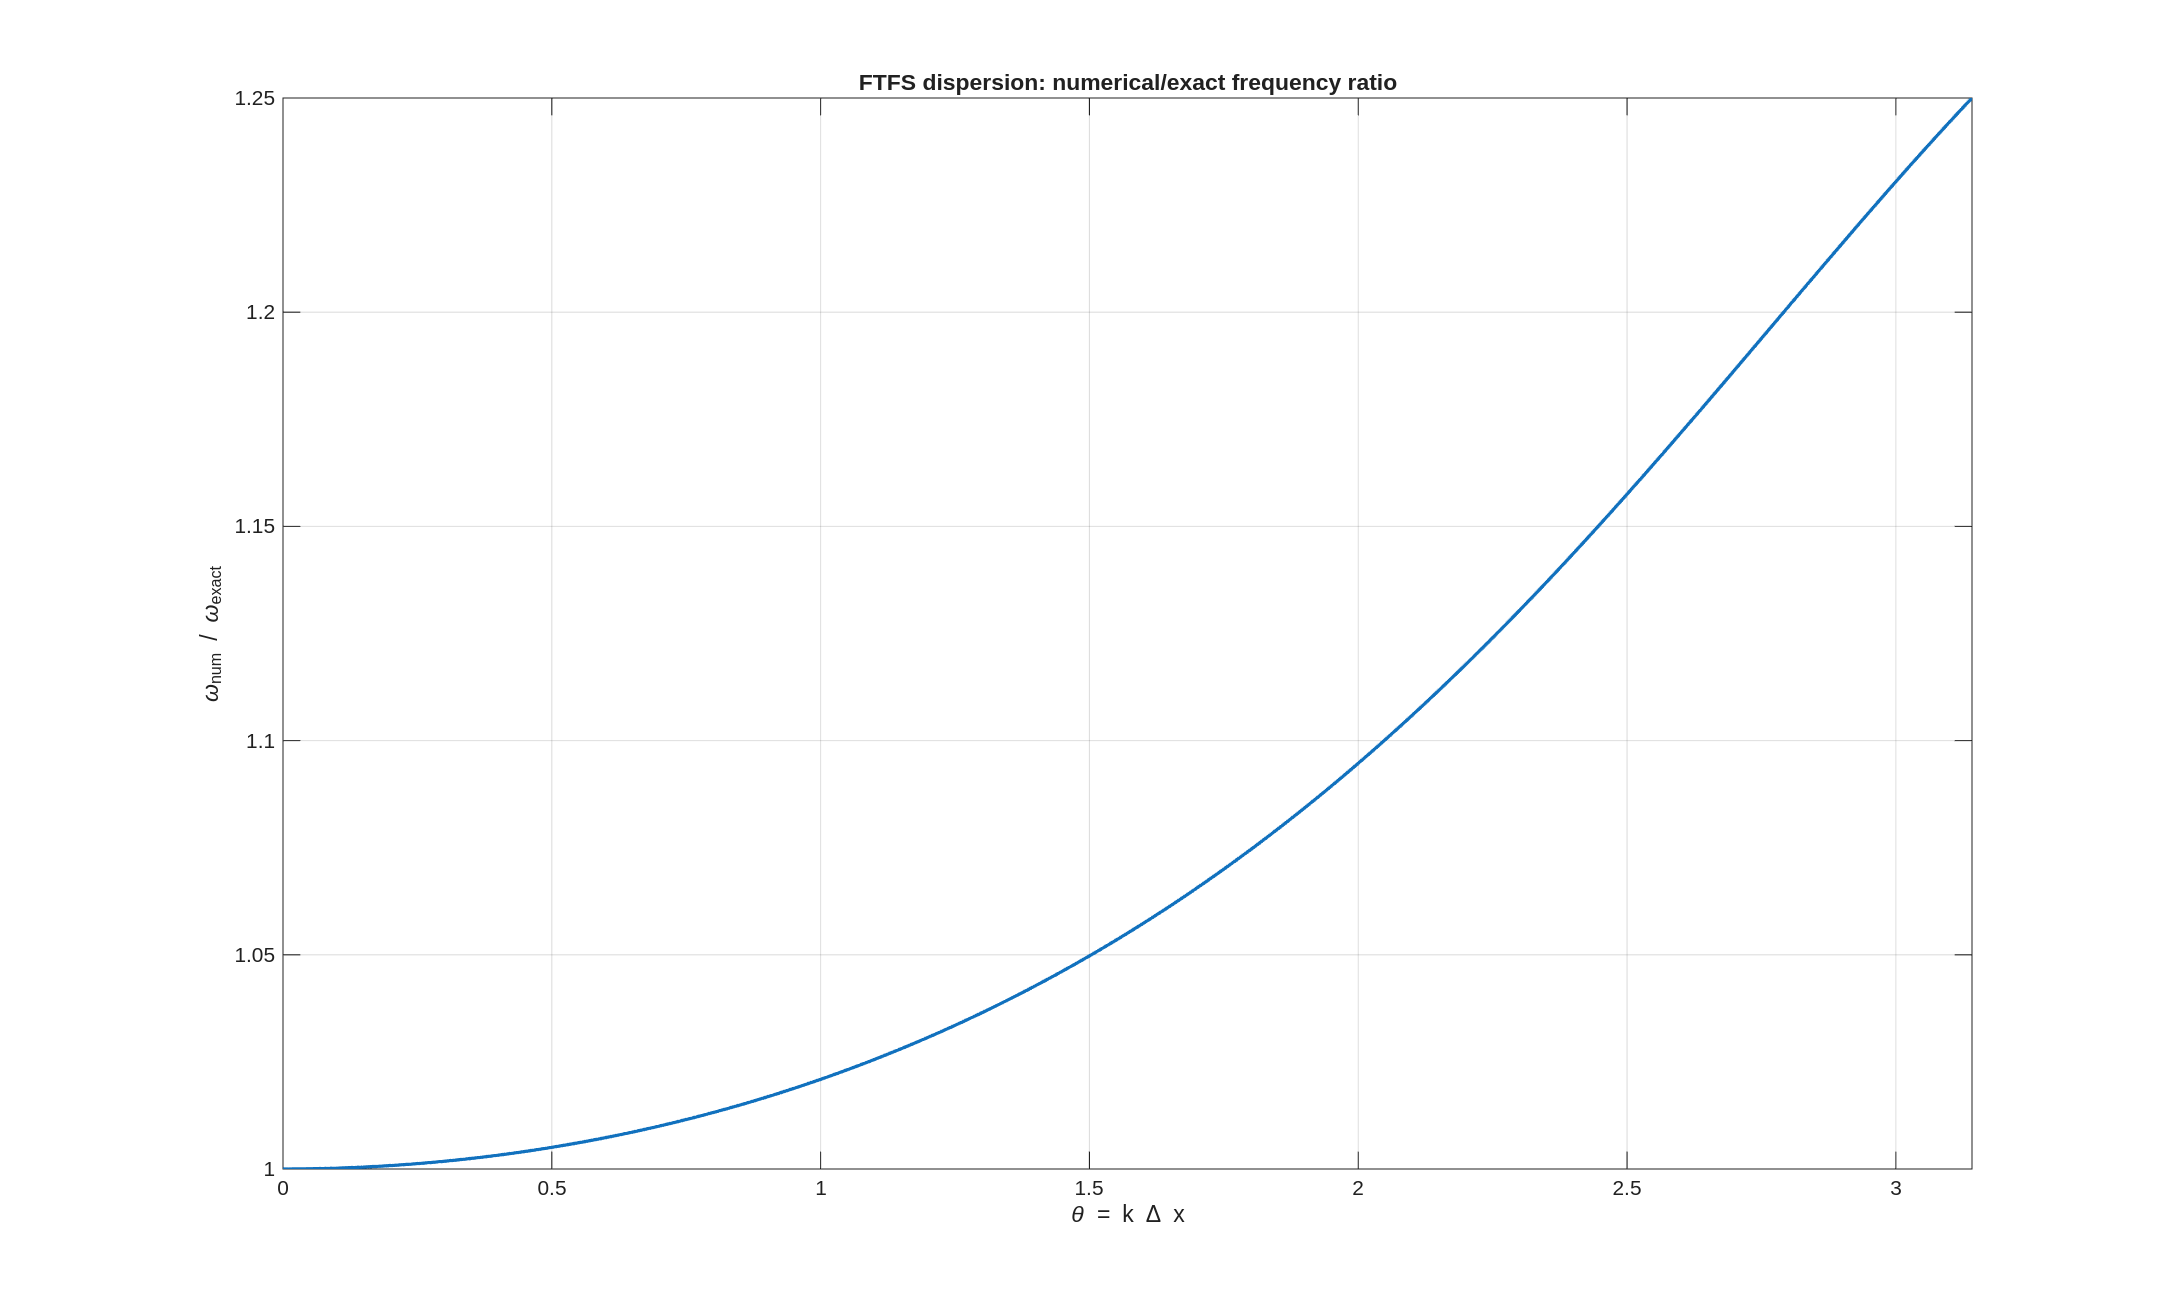
\includegraphics[scale=0.4]{DispersionCurve.png}
			\caption{FTFS Dispersion Curve}
			\label{fig:DispersionCurve}
		\end{figure}

		$\hat{\omega}$ is time dependent indicating that the dispersion will be increasing over successive iterations, progressively reducing accuracy.  The code for Figure \ref{fig:DispersionCurve} and Figure \ref{fig:DissipationCurve} is
		\lstinputlisting{DispDesp.m}

		\break
		\begin{figure}
			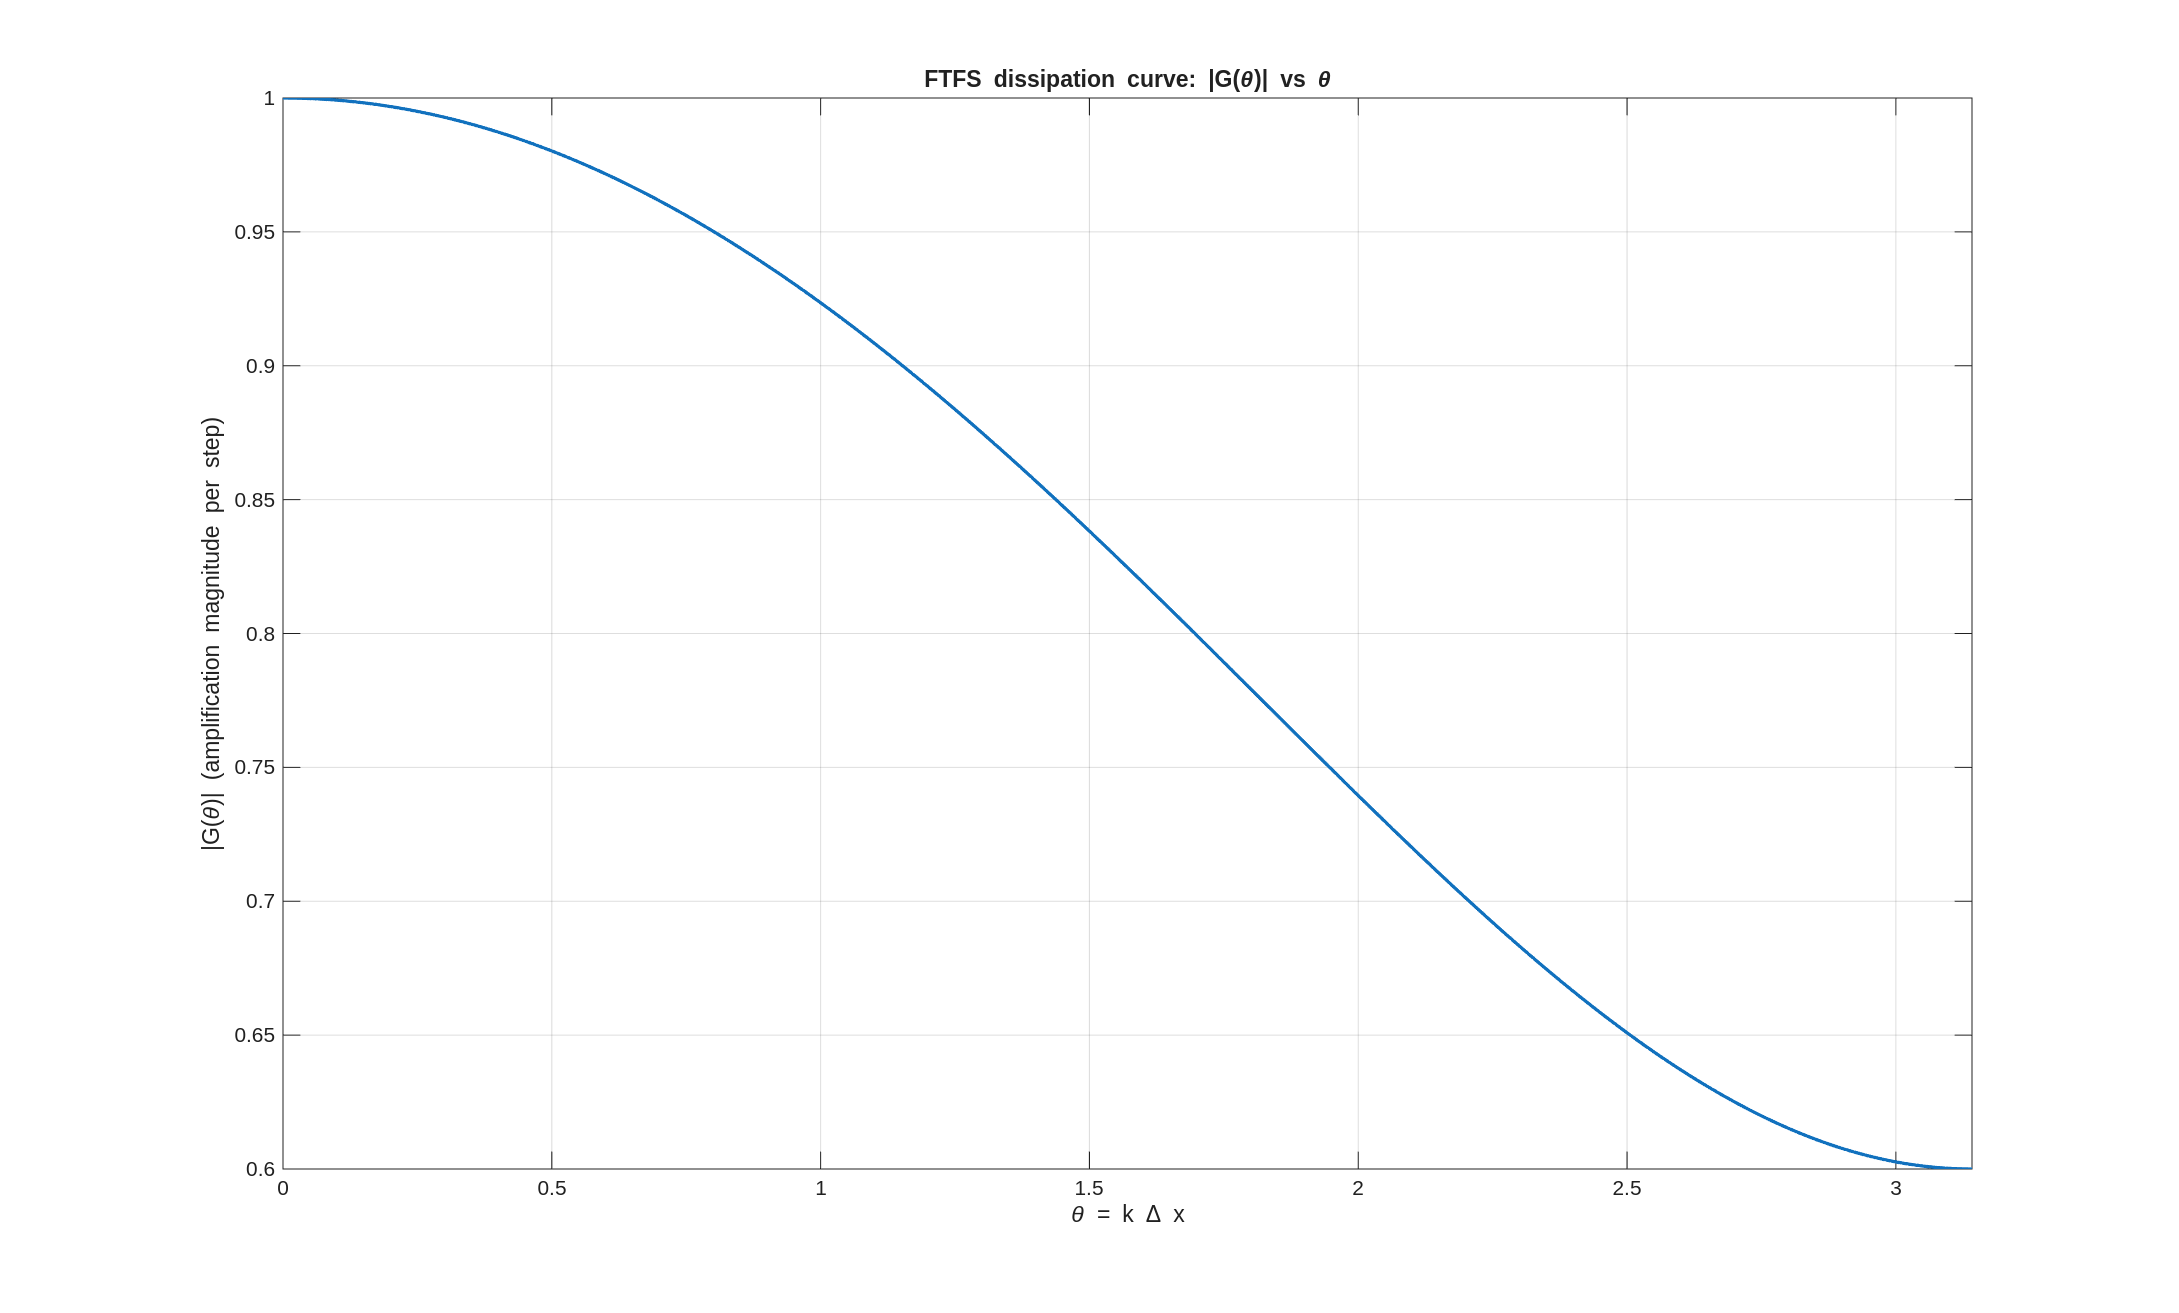
\includegraphics[scale=0.4]{DissipationCurve.png}
			\caption{FTFS Dissipation Curve}
			\label{fig:DissipationCurve}
		\end{figure}
		
		This curve compares the dissipation to the wave number.  A one indicating no dissipation.  Thus the higher the wave number less accurate the numeric solution reflects the analytic solution.
	\end{description}
	
	\item \textbf{Change the initial conditions}

	\textbf{Part (b)} of the assignment is: For the initial condition $u(x,0) = \sin^{40}(\pi x)$, plot the analytical and numerical solution at time $t=1$, quantify the amount of dissipation.\\
	
	\begin{figure}
		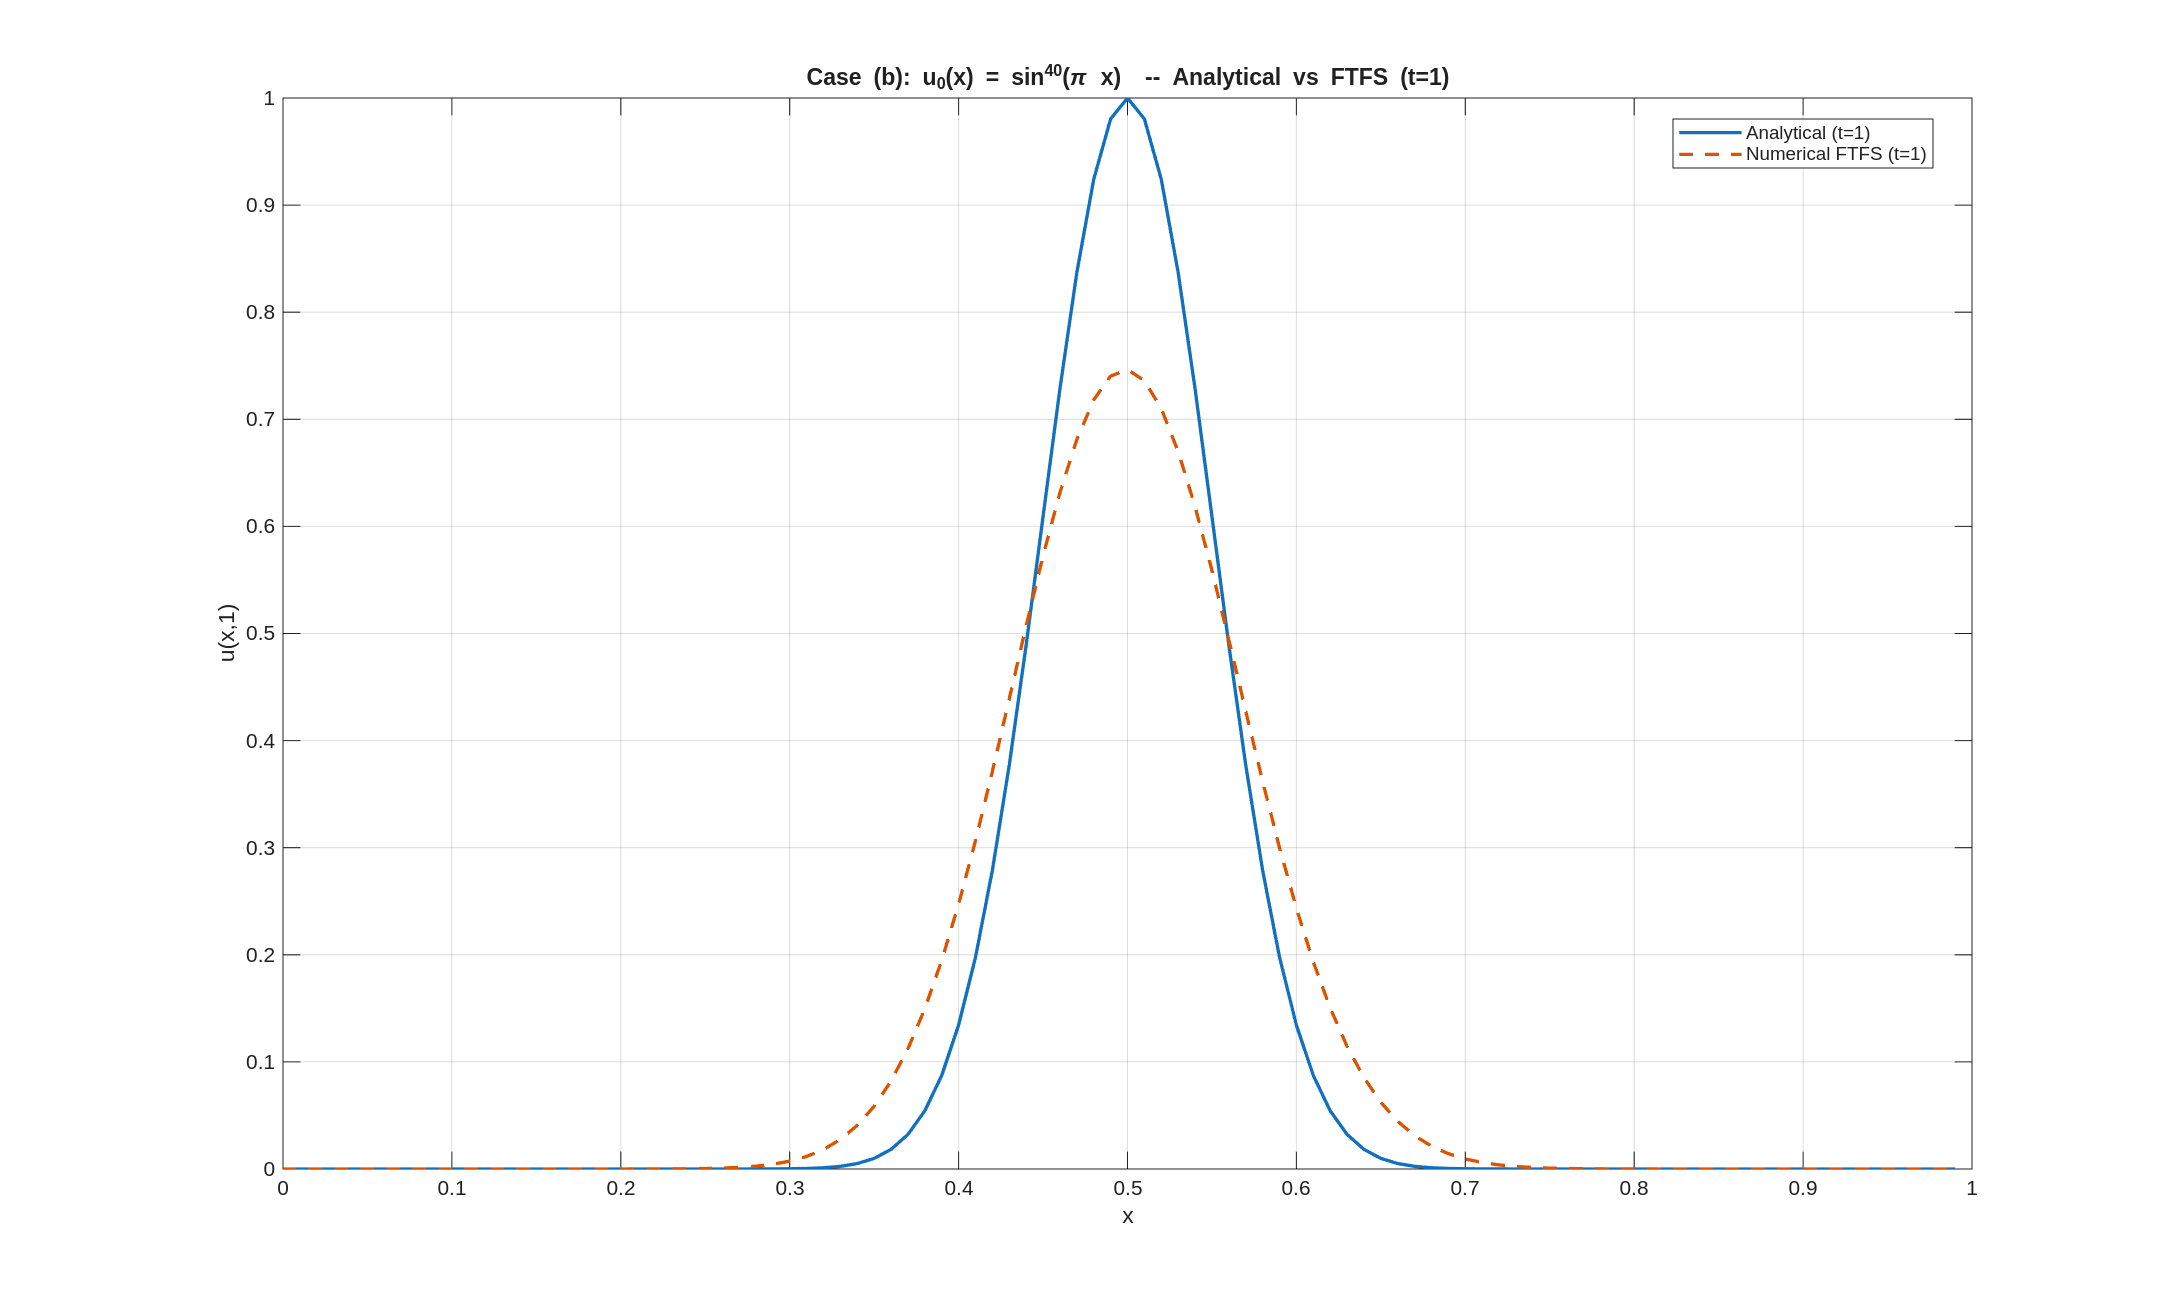
\includegraphics[scale=0.4]{ExactSolution_b.png} 
		\caption{Changing the function from $\sin^{20}(\pi x)$ to $\sin^{40}(\pi x)$}
		\label{fig:ChangeInitialConditions}
	\end{figure}	
	
	As compared to Figure $\ref{fig:Graph1}$ we can see that the shape of the wave is much narrower for both the analytic solution and the numeric solution.  And, by observation, the difference in maximum amplitude remains the same, indicating a similar dissipation factor.
	
	\textbf{Part (c)} of the assignment is: Change the initial condition to $u(x,0)=1$ for $0.4\le x \le 0.6$ and $u(x,0)=0$ otherwise.  Plot the analytical and numerical solution at time $t=1$, quantify the amount of dissipation.  That is, the initial conditions $t=0$ are
	\begin{align*}
		u(x,0) &= \BINDEF{1 & 0.4 \le x \le 0.6}{0 & \text{otherwise}}
	\end{align*}

	\begin{figure}
		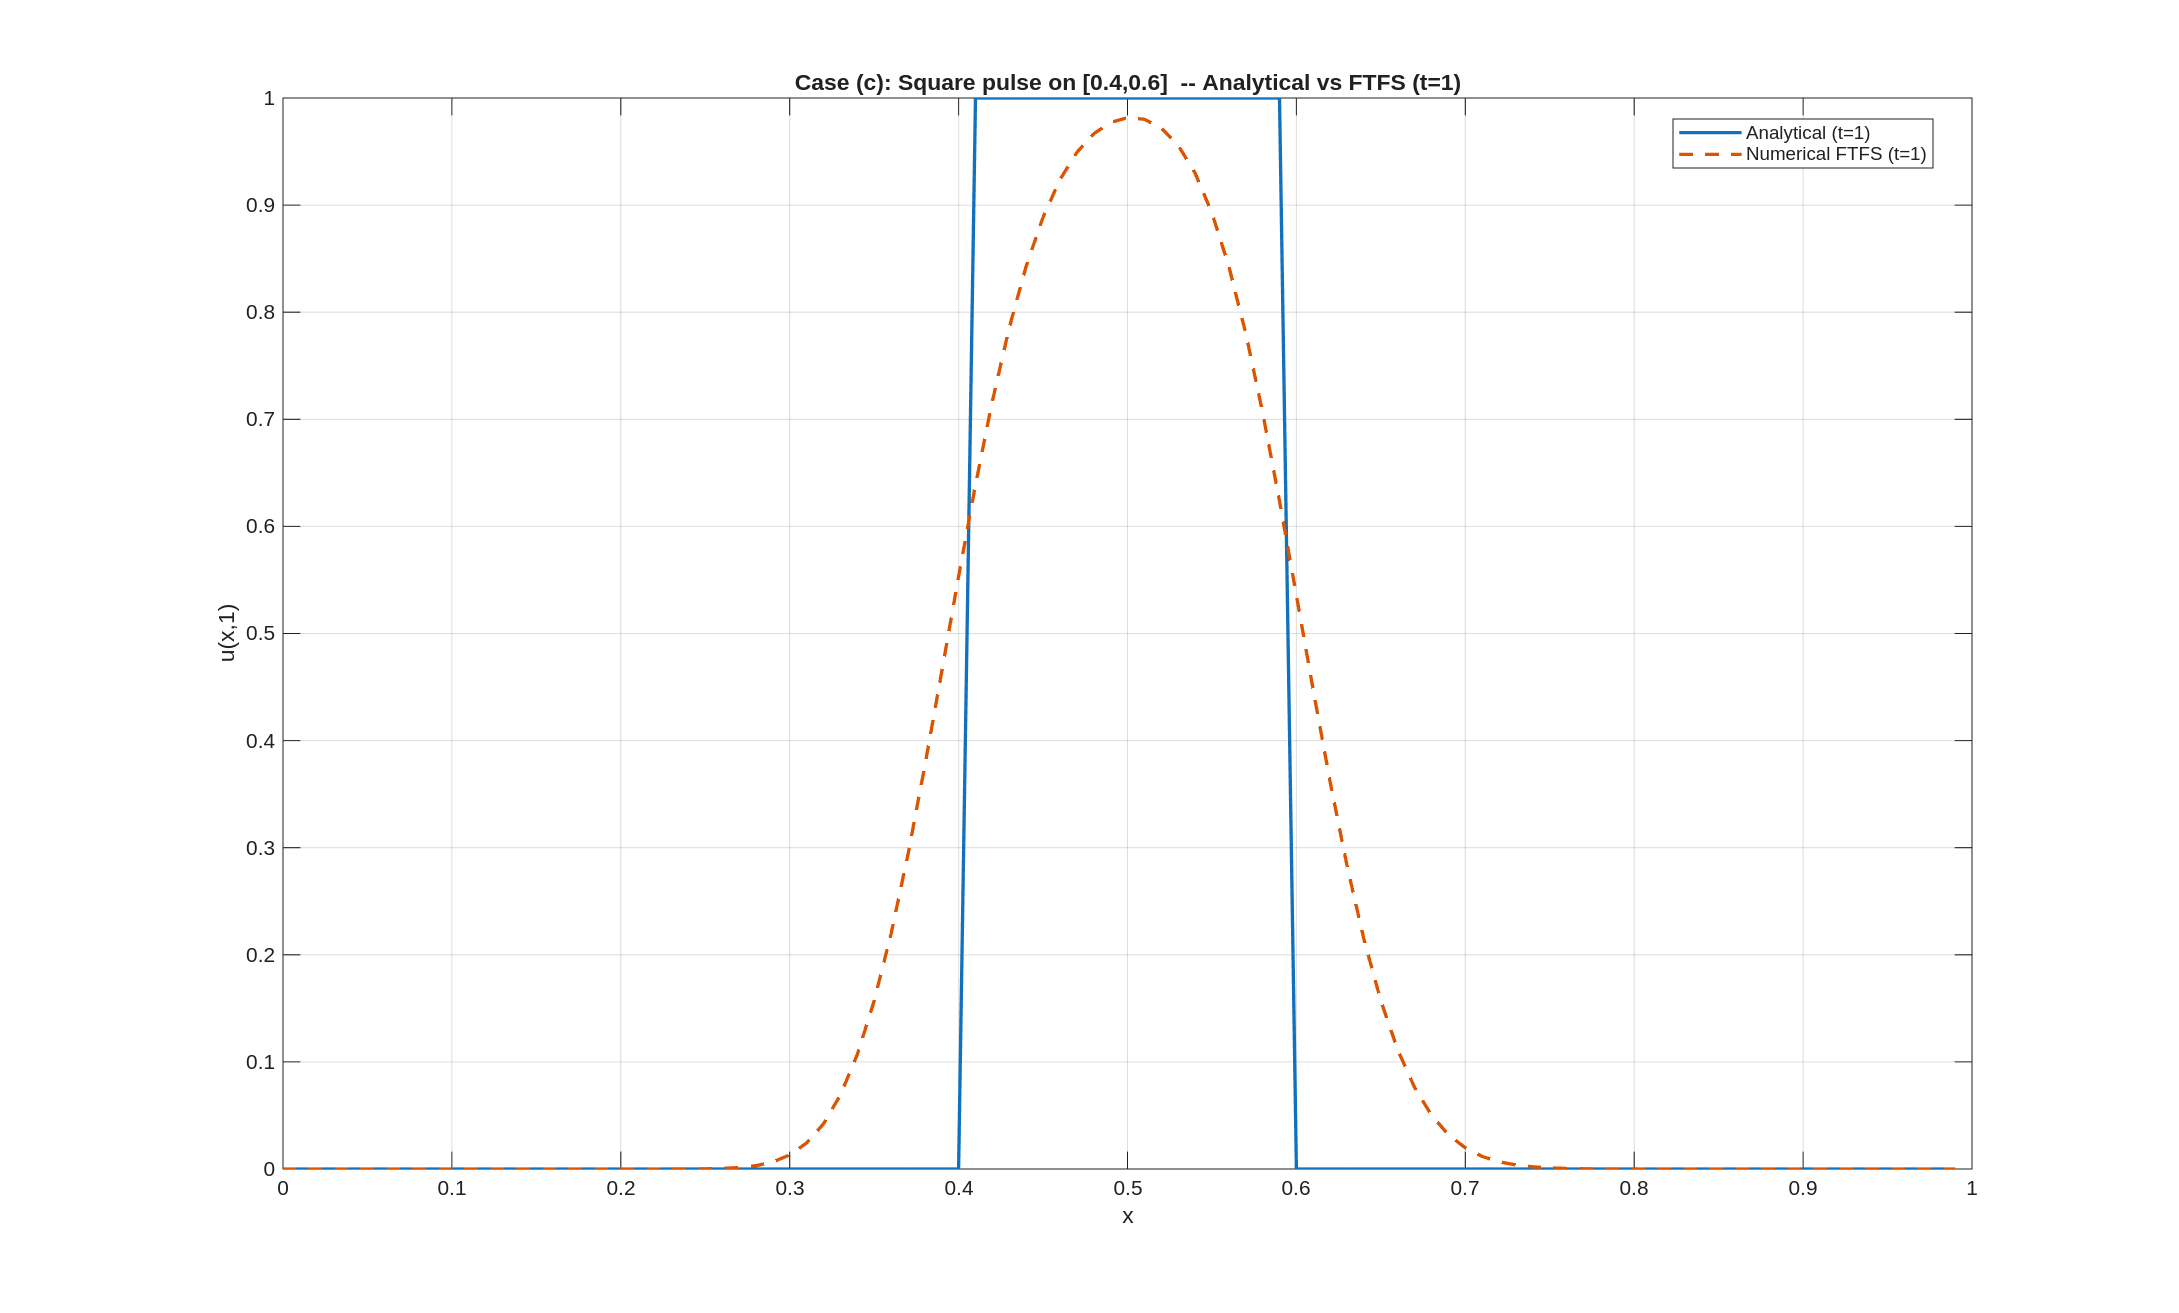
\includegraphics[scale=0.4]{ExactSolution_c.png} 
		\caption{Changing the function from to a step function on $[0.4, 0.6]$}
		\label{fig:ChangeInitialConditions}
	\end{figure}
	
	\textbf{Comparing the $\sin^{40}(x)$ example to the Square Pulse Example}
	
	The primary question is ``How much of the wave amplitude was reduced by the numerical method?"  This translates to a fraction dissipation, $D$.
	\begin{align*}
		D &= \frac{|u(t)|-|\hat{u}(t)|}{|u(t)}
	\end{align*}where $u$ is the exact solution and $\hat{u}$ is the numeric solution. \\
	
	Resulting in the following information:\\ \\
	\begin{tabular}{|c|c|c|c|}
		\hline & $E(0)$ & $E(1)$ & $D$ \\
		\hline (b) & 0.0889 & 0.0662 & 0.259 \\
		\hline (c) & 0.21 & 0.159 & 0.239\\
		\hline
\end{tabular}	\\ \\
	Where $E$ is the comparative energy and $D$ is the fractional dissipation.  Thus the energy per amplitude drop off for (b) is $25\%$ and for (c) it is $23.9\%$	
		
	\newpage
	\item \textbf{Power Spectrum Density Analysis}
	
	Since the PDE requires a periodic solution, understanding the component waves is essential.  Power Spectrum Analysis helps in this regard by indicating which wave forms dominate over the solution.  The process is to take the vector numeric solutions and use the Fast Fourier Transform to generate a vector of complex values representing the wave numbers.  We then compare the square of these values (being complex, the square provides us with real values for comparison).  Figure $\ref{fig:PSDGraph}$ displays this comparison.  \\
	
	We can see that a Square Pulse requires many wave forms in order to approximate the solution (which is to be expected).  In contrast, the sinusoidal wave uses only a few intitial wave numbers while the remaining drop off completely.  Since different wave numbers travel at different speeds we can expect the Square Wave impulse have strong dispersion.  Where as the sinusoidal solution will have fewer strong wave numbers and correspondingly  less dispersion.  
		\begin{figure}
		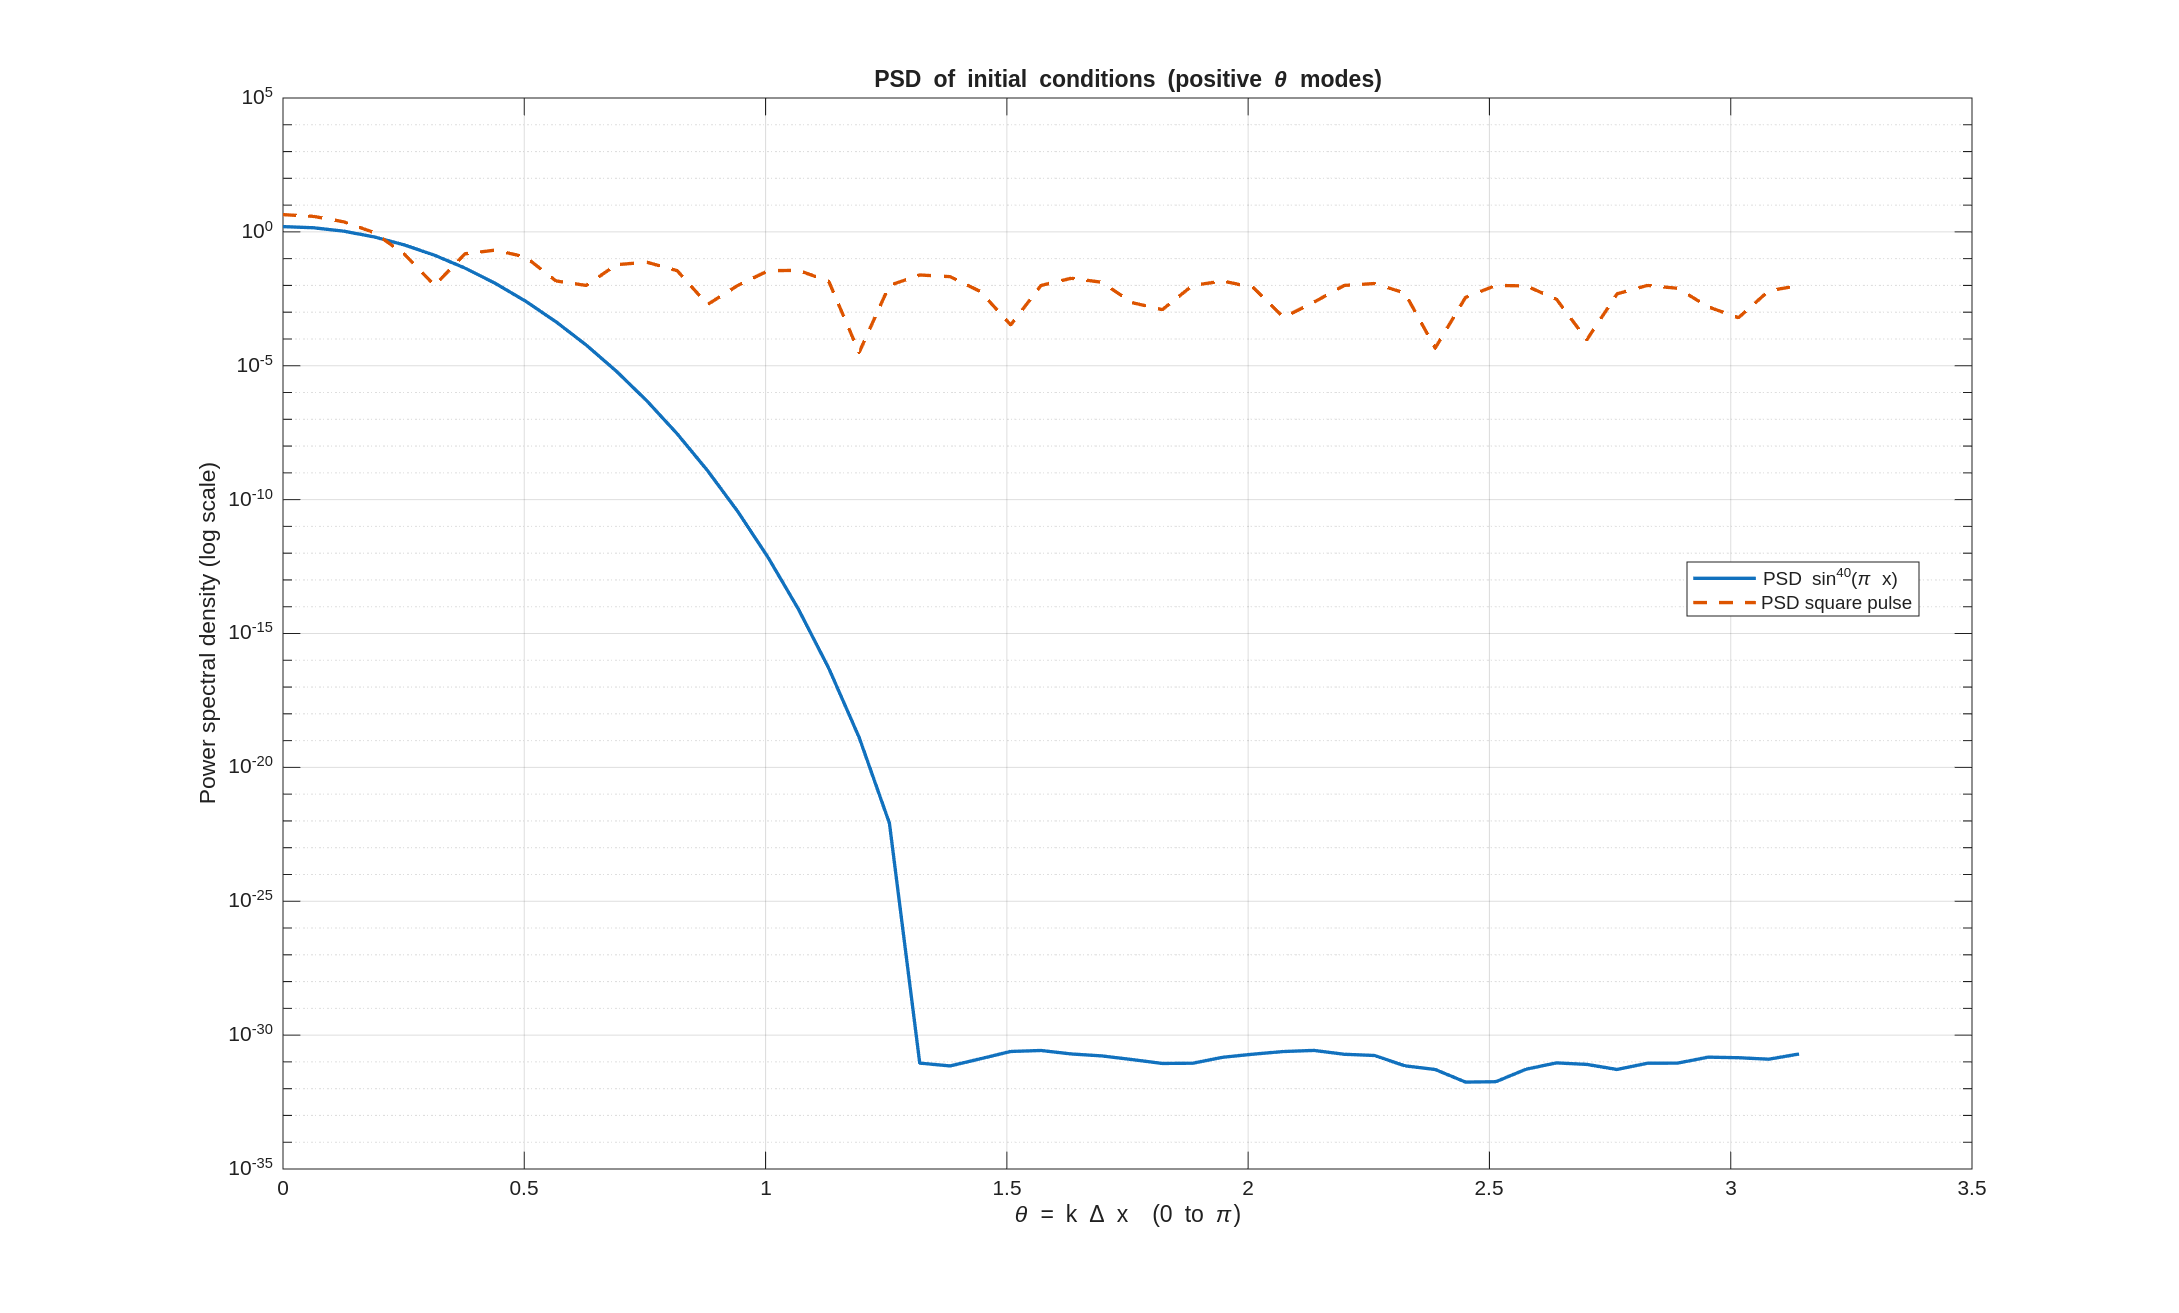
\includegraphics[scale=0.4]{PSD.png} 
		\caption{Power Spectrum Density of FTFS for $\sin^{40}(x)$ and a Square Pulse}
		\label{fig:PSDGraph}
	\end{figure}
\end{description}
	
	The code for this comparison and PSD analysis is 
	\lstinputlisting{Compare_b_c.m}

\newpage

\begin{center}
	\textbf{\Large{Apply the Leap Frog scheme to the\\ Transportation Equation with Periodic Boundary Conditions}}
\end{center}

\begin{description}
	\item \textbf{Leap Frog: }
	
	We start in the same way as FTFS, that is, by dividing the time and space domains into subintervals.  However, instead of using using the next element to determing both the partial derivatives, we use the element above and below.  Thus, we get these two partial derivatives for the time and space dimensions.
	\begin{align*}
		\PART{u}{t} &\approx \frac{u_j^{n+1}-u_j^{n-1}}{2\Delta t} & \quad  \PART{u}{x} &\approx \frac{u_{j+1}^n-u_{j-1}^{n}}{2\Delta x}
	\end{align*}Inserting these into the Transport Equation we get
	\begin{align*}
		\frac{u_j^{n+1}-u_j^{n-1}}{2\Delta t} &= \frac{u_{j+1}^n-u_{j-1}^{n}}{2\Delta x}\\
		u_j^{n+1} &= u_j^{n-1} -\lambda(u_{j+1}^n-u_{j-1}^n),
	\end{align*}where $\lambda = \Delta t/\Delta x$.
		
	We analyze \textbf{disperstion and dissipation} again by the use of Fourier Transforms.  Inserting $u_j^n = G^ne^{ij\theta}$ where $\theta = n\Delta x$ and we get
	\begin{align*}
		G^2 &= 2i\lambda \sin \theta G-1 = 0 \\
		G(\theta) &= \sqrt{1-\lambda^2 \sin^2\theta} - i \lambda \sin \theta \\
		|G(\theta)| &= 1
	\end{align*}which indicates \textit{no dissipation}. Dispersion, however, changes with respect to time (as outlined in great detail in "Finite Difference" by Le Veque, page 223).

		\begin{figure}
		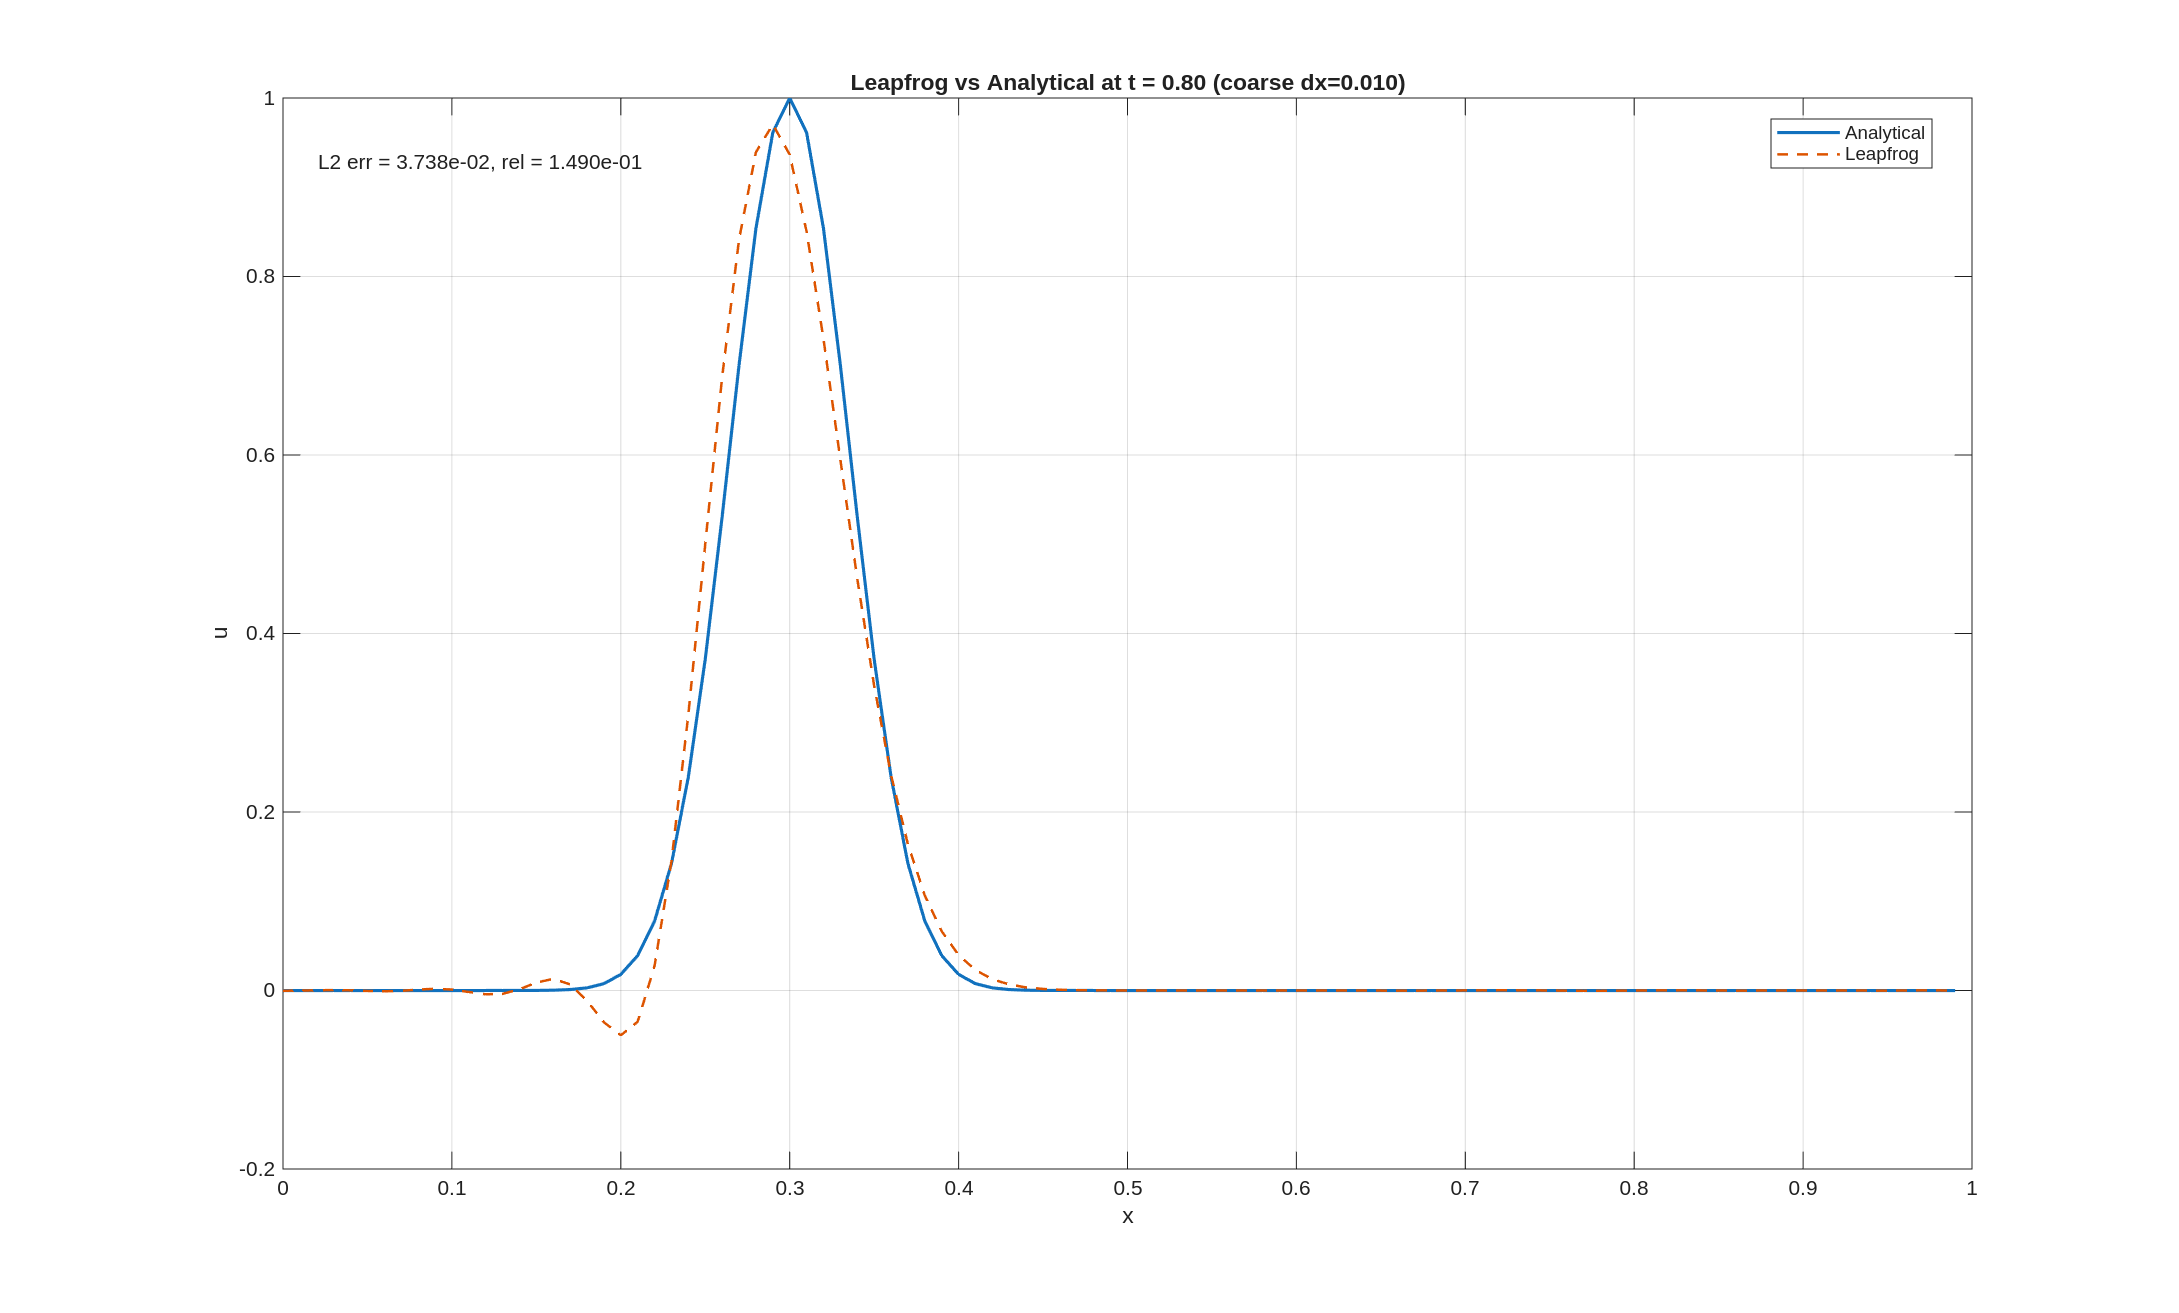
\includegraphics[scale=0.4]{LeapFrogGraph.png} 
		\caption{Leap Frog Graph for $\sin^{80}(x)$ at $t=0.8$}
		\label{fig:LeapFrogGraph}
	\end{figure}
		\begin{figure}
		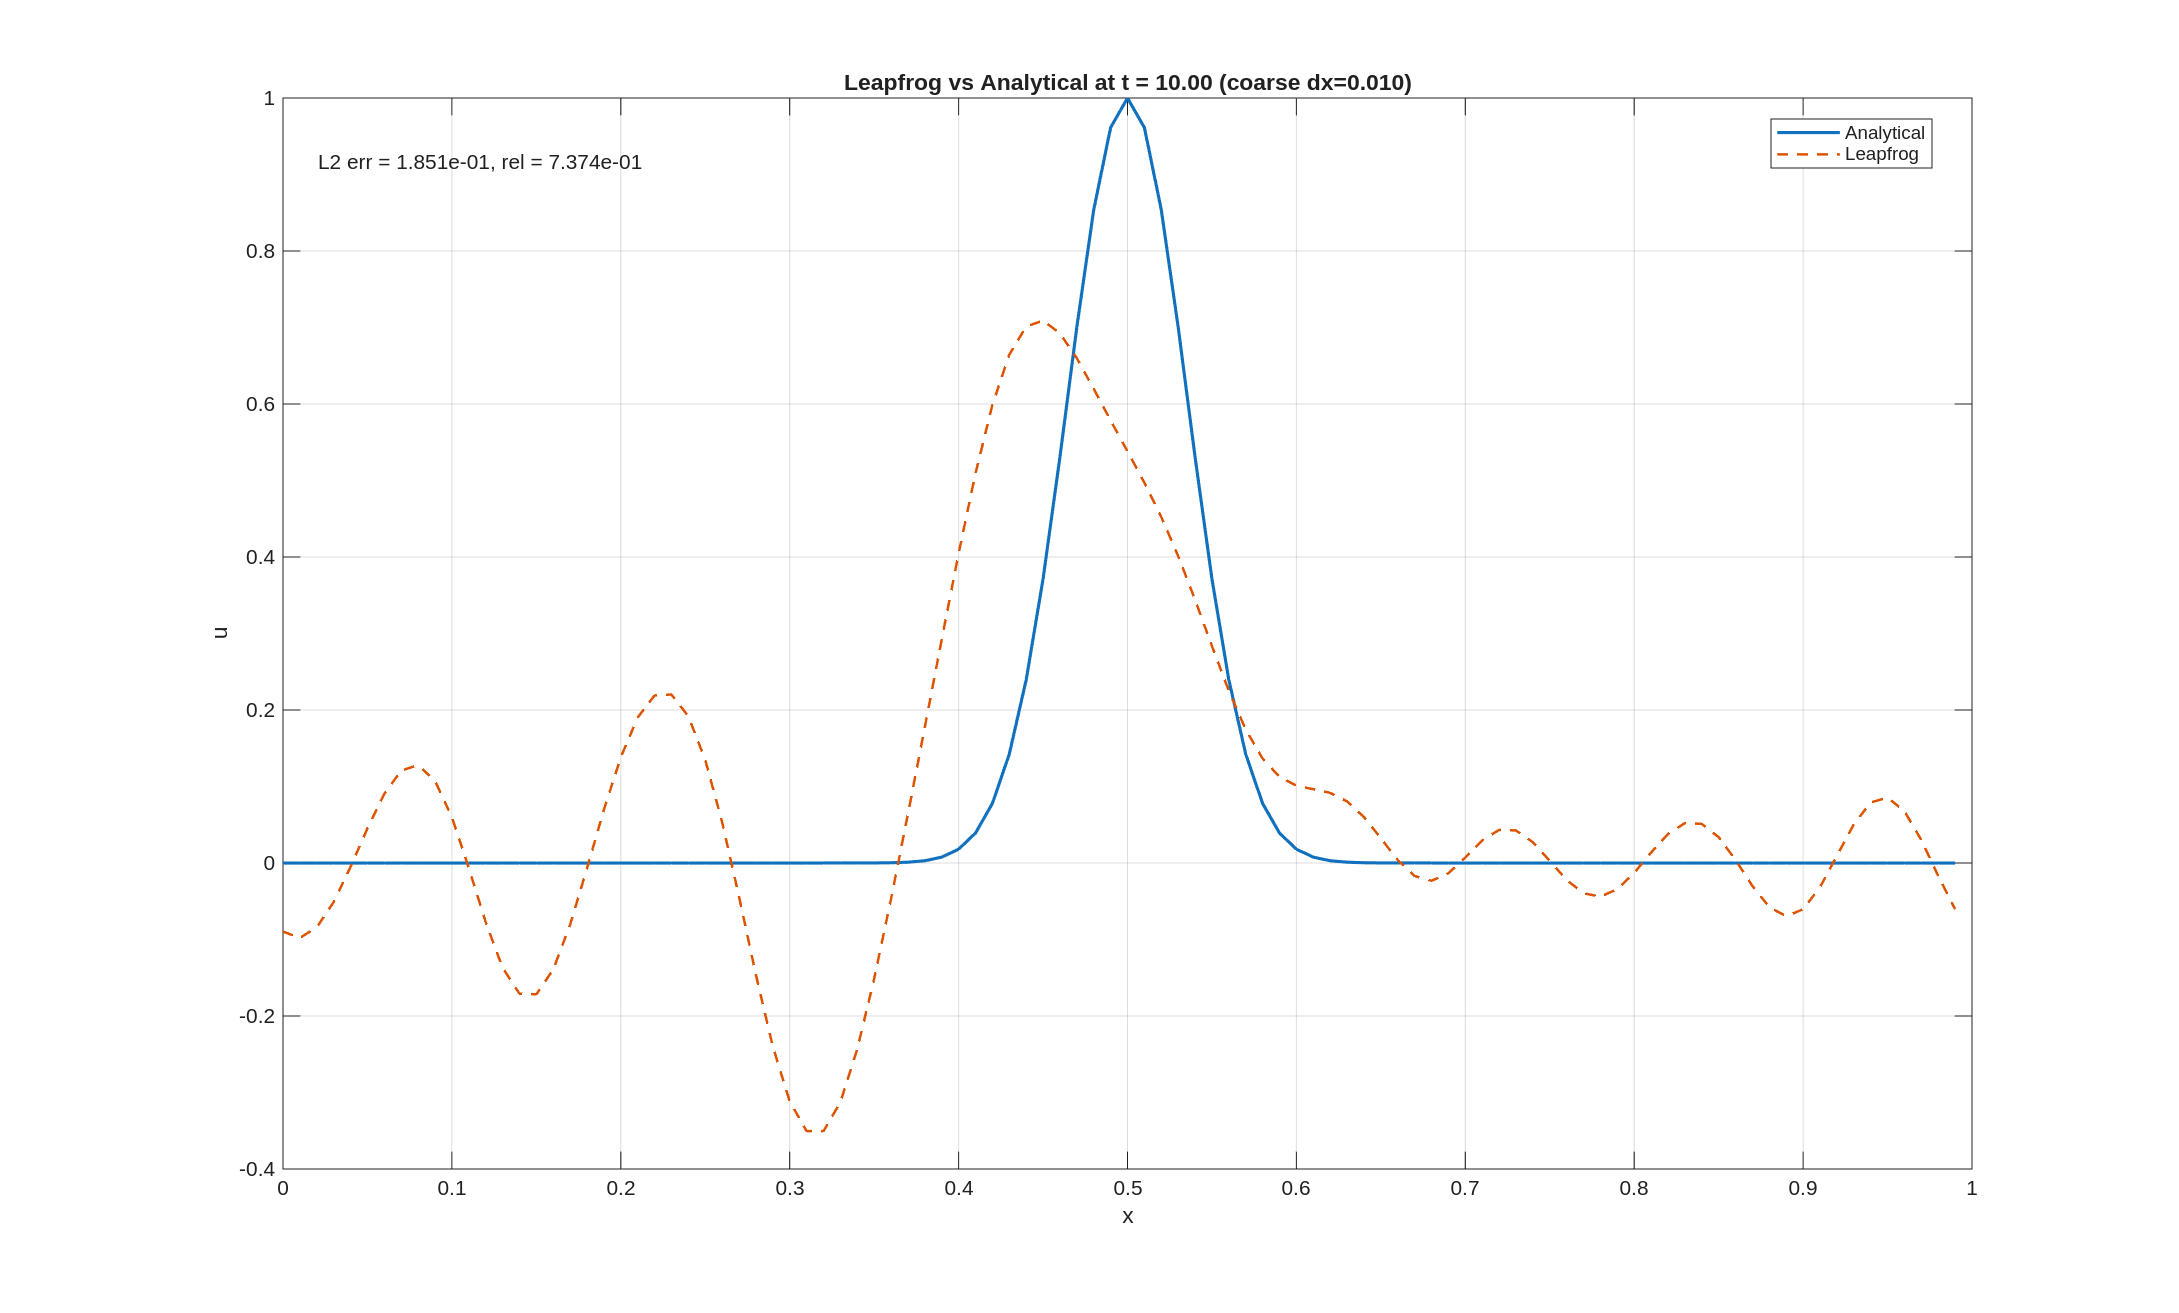
\includegraphics[scale=0.4]{LeapFrogGraph2.png} 
		\caption{Leap Frog Graph for $\sin^{80}(x)$ at $t=10$}
		\label{fig:LeapFrogGraph}
	\end{figure}
		\begin{figure}
		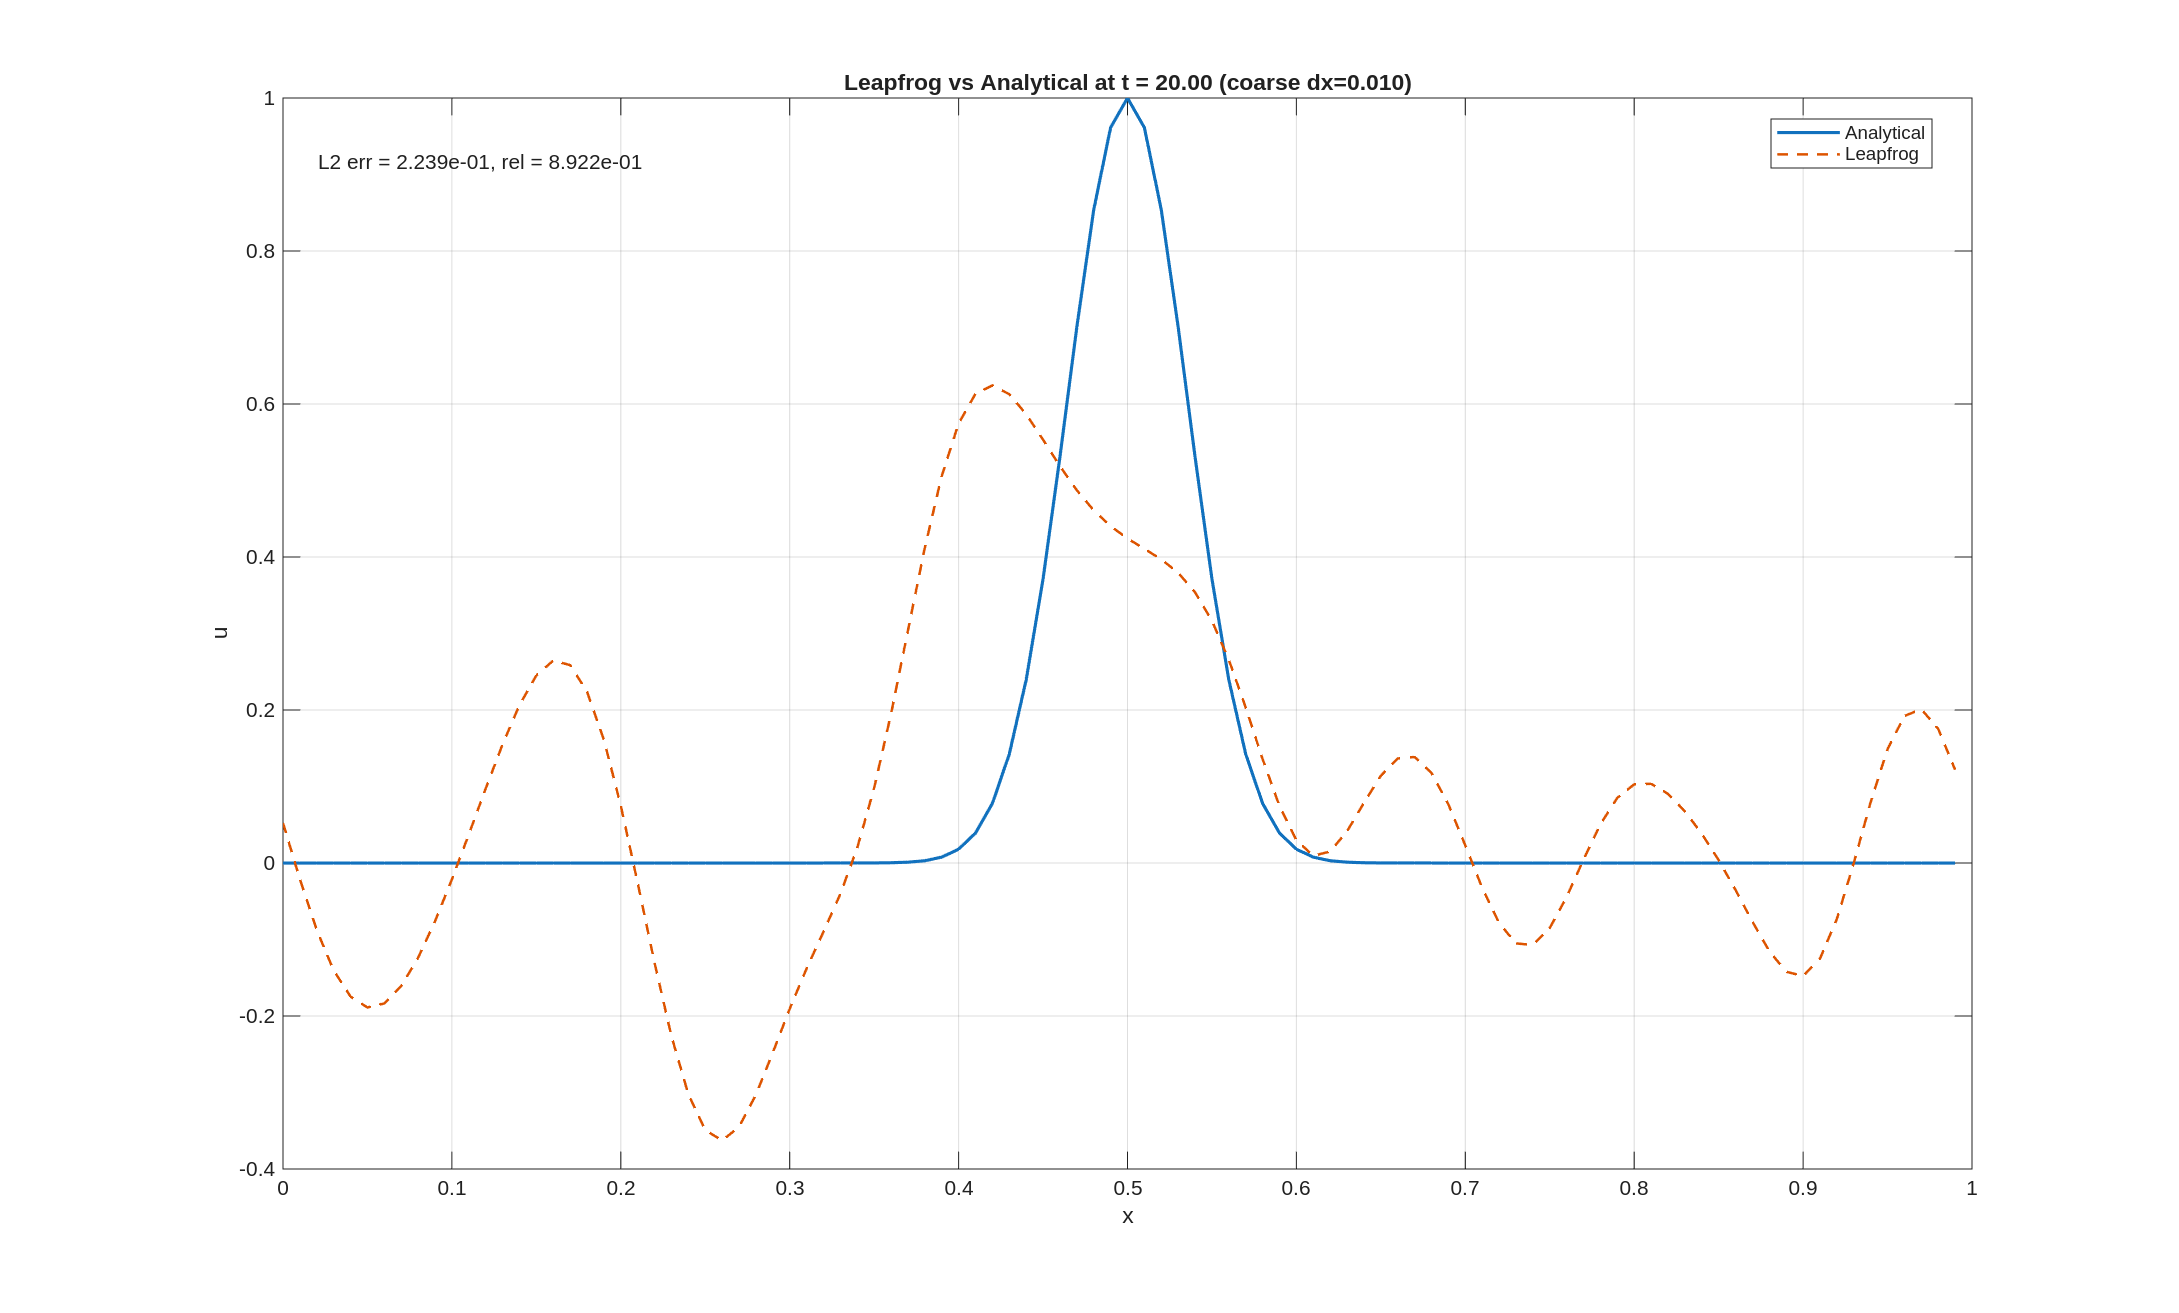
\includegraphics[scale=0.4]{LeapFrogGraph3.png} 
		\caption{Leap Frog Graph for $\sin^{80}(x)$ at $t=20$}
		\label{fig:LeapFrogGraph}
	\end{figure}
	
	Examining Figure 7 through Figure 9 we can see the effects of the dispersion over increasing values of $t$.  Note that these graphs focus on low frequency wave numbers.
	
	\newpage
	\item \textbf{Power Spectrum Density Analysis}
	
	As described above in FTFS, Power Spectrum Density Analysis helps establish how accurate the numerical solution is in comparison with the analytic solution.  We further anbalyze the 'coarse' frequency modes (long wavelengths and low frequency) with the 'refines' frequency modes (short wavelengths and high frequency). We can see from Figure 10 there is a distinct difference between these to categories of wave numbers noting that 'coarse'/lower frequences dominate the numeric solutions sigfnificatnly over the 'refined'/higher frequencies, supporting what is seen in Figure 7 through Figure 9.
	\begin{figure}
		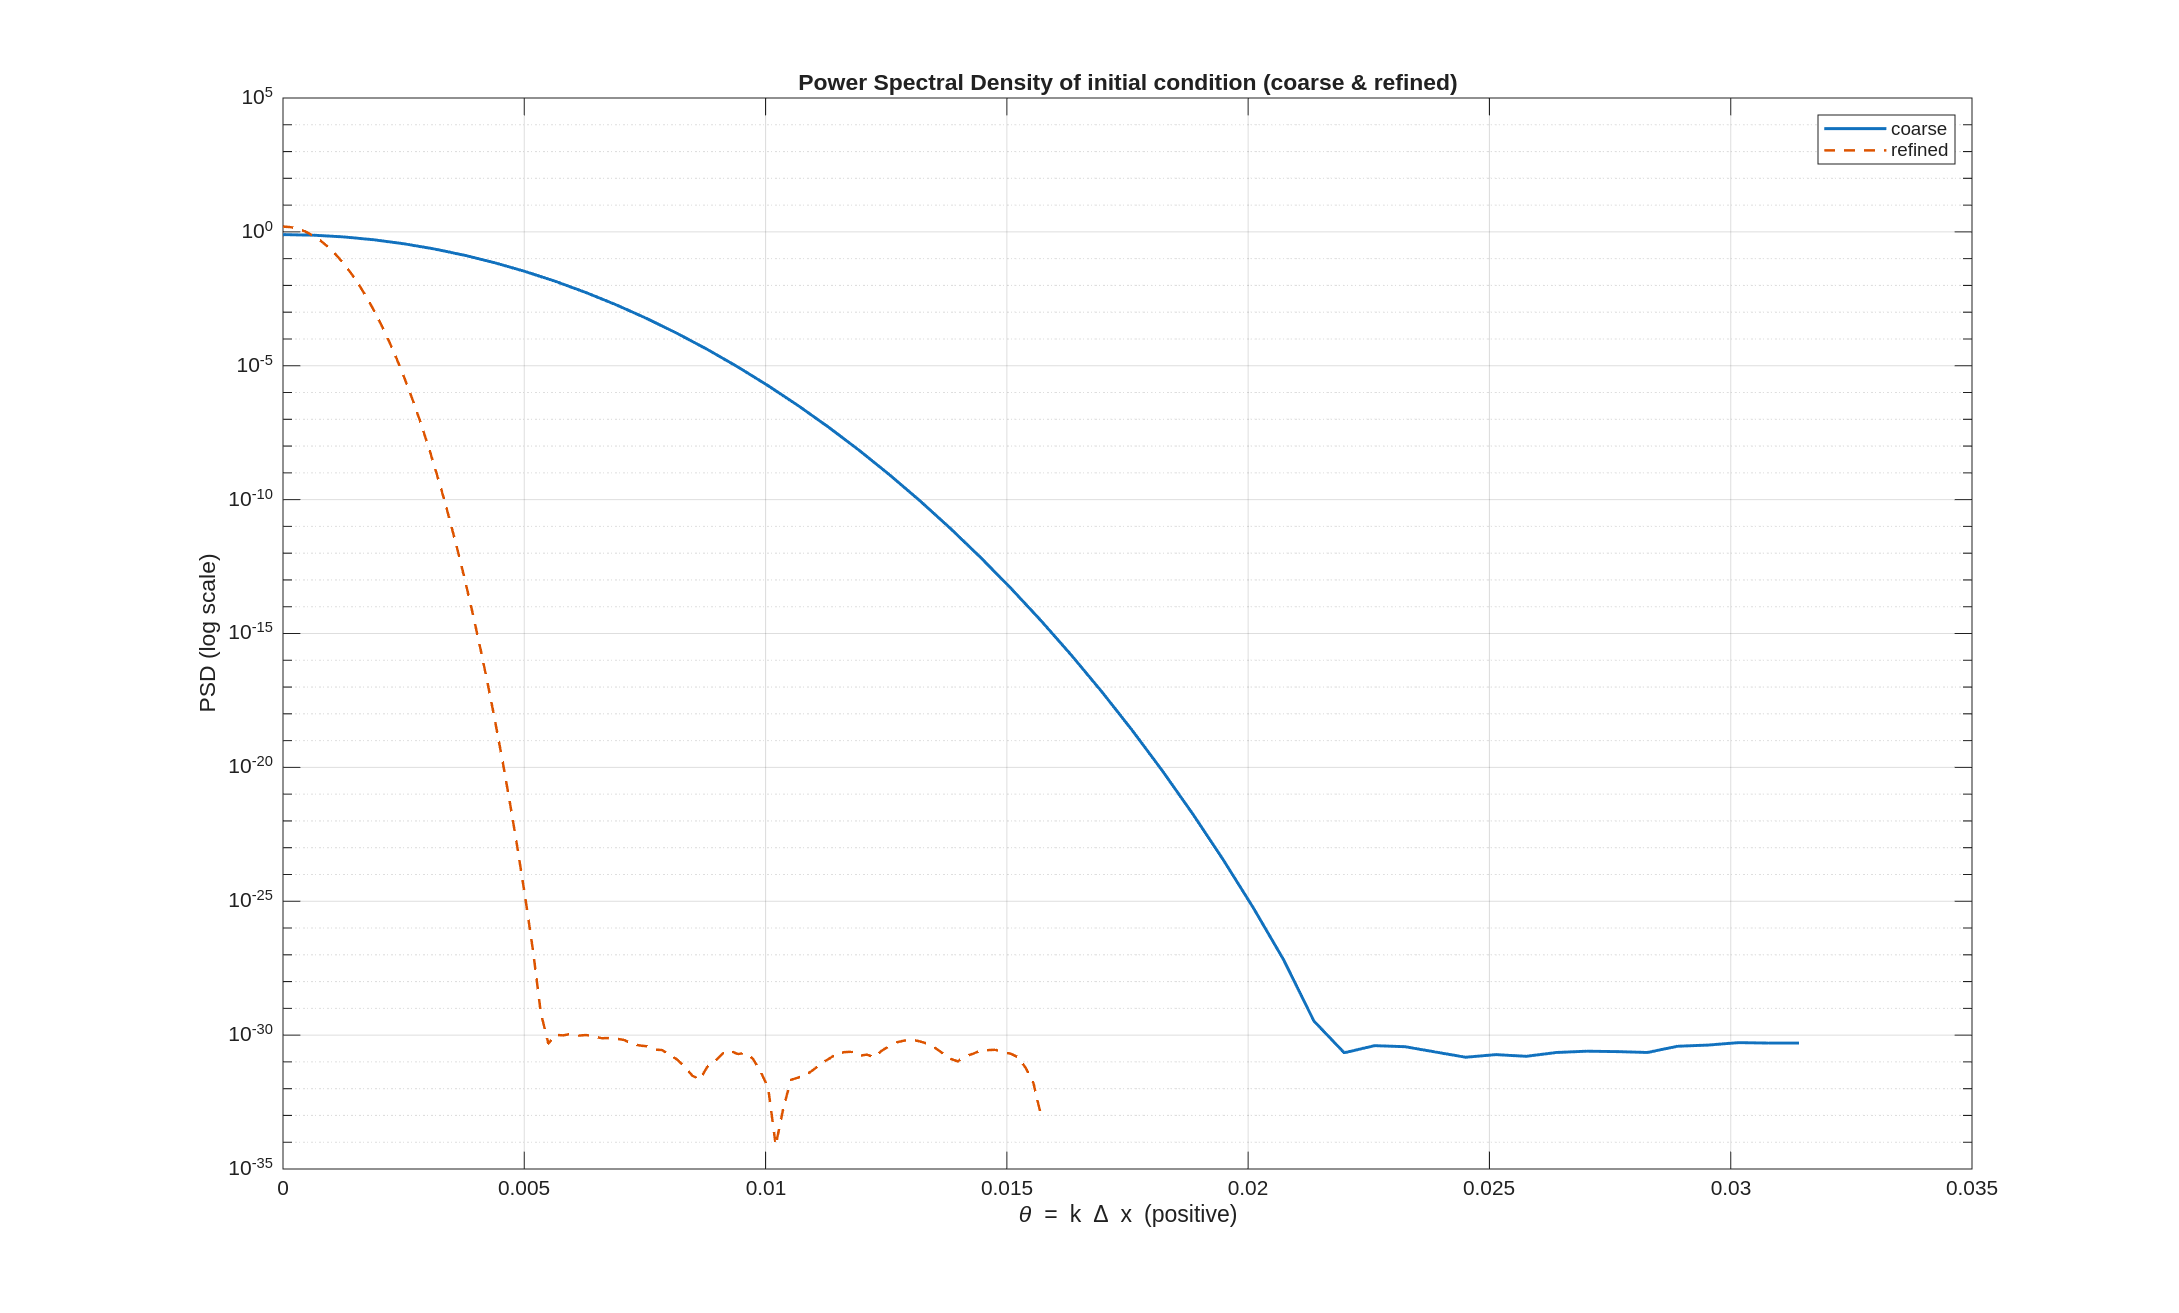
\includegraphics[scale=0.4]{PSD_LeapFrog.png} 
		\caption{PSD on Leap Frog Scheme Anlaytic vs Numerical solutions}
		\label{fig:PSDLeapFrog}
	\end{figure}

	The following is the MatLab code for all graphs and calculations.
		\lstinputlisting{LeapFrog2.m}

\end{description}

\end{document}